%% V1.0
%% by Gabriel Garcia, gabrcg@gmail.com
%% This is a template for Udacity projects using IEEEtran.cls

%% Be Udacious!

\documentclass[10pt,journal,compsoc]{IEEEtran}

\usepackage[pdftex]{graphicx}    
\usepackage{cite}
\usepackage[inline]{enumitem}
\usepackage{hyperref}
\usepackage{algorithmic}
\usepackage{algorithm}
\hyphenation{op-tical net-works semi-conduc-tor}


\begin{document}

\title{Where Am I?}

\author{Saminda Abeyruwan}

\markboth{Where Am I project, Robotic Nanodegree, Udacity}%
{}
\IEEEtitleabstractindextext{%

\begin{abstract}

Mobile robot localization estimates the robot pose relative to a given map of the environment. This project empirically evaluates the Adaptive Monte Carlo Localization algorithm using Gazebo simulator and Rviz visualizer. Using ROS framework, a baseline two- and custom four-wheeled mobile robot platforms with senors have been developed. The robots have used ROS amcl and navigation stack packages for global localization and path planning. By tuning the amcl and planner parameters, the robots have been localized on the map and successfully navigated to predefined target locations. 
\end{abstract}

% Note that keywords are not normally used for peerreview papers.
\begin{IEEEkeywords}
Robot, IEEEtran, Udacity, \LaTeX, deep learning.
\end{IEEEkeywords}}


\maketitle
\IEEEdisplaynontitleabstractindextext
\IEEEpeerreviewmaketitle
\section{Introduction}
\label{sec:introduction}

\IEEEPARstart{M}{bile} robot localization estimates the robot pose relative to a given  map of the environment \cite{Thrun:2005:PR:1121596}. Given the coordinates of the map, a robot pose, $x_t = (x~ y~\theta)^T$, sufficiently determines location and orientation of the robot. The robot pose cannot be directly sensed, and it must be inferred from the noisy sensor data over time. There are four dimensions with which the complexity of the localization problems can be analyzed. 

The first dimension is based on the knowledge available initially, and during the operation time.  There are three complexity classes; \begin{enumerate*} \item \textit{position tracking}, the initial pose of the robot is known, and the localization is achieved via accommodating the noisy robot motion. If the motion error is relatively small, the pose uncertainty is often approximated by a unimodal distribution.  This is also a local localization, as the pose is confined to a small region of the robot true pose, \item \textit{global localization}, the initial pose of the robot is unknown, and it is inferred from relative to a known map of the environment. The problem is  more difficult than position tracking, and generally cannot be bounded by a a unimodal distribution, and \item \textit{kidnapped robot problem}, the robot gets teleported to some other location. The robot needs to reevaluate its pose, and recover from such situations to exhibits truly autonomous capabilities. \end{enumerate*} 

The second dimension addresses the nature of the environment: \begin{enumerate*} \item \textit{static environments}, the objects in the environment remain static, and the only variable is the robot pose, and \item \textit{dynamic environments}, contains objects whose location of configuration changes overtime.  \end{enumerate*}

The third dimension addresses the ability of the localization algorithms to control the motion of the robot. There are two modes: \begin{enumerate*} \item \textit{passive localization}, where the localization module only observes the sensor and motion readings, and the robot is controlled by another set of modules, and \item \textit{active localization}, controls the robot to minimize the localization error.  \end{enumerate*} 

Finally, last dimension involved the number of robots involved: \begin{enumerate*} \item \textit{single-robot localization}, all sensor and motion information is collected from a single robot platform, and \item \textit{multi-robot localization}, information from other robots in a team of robots are used to solve the localization problem. \end{enumerate*}

\begin{figure}[thpb]
      \centering
      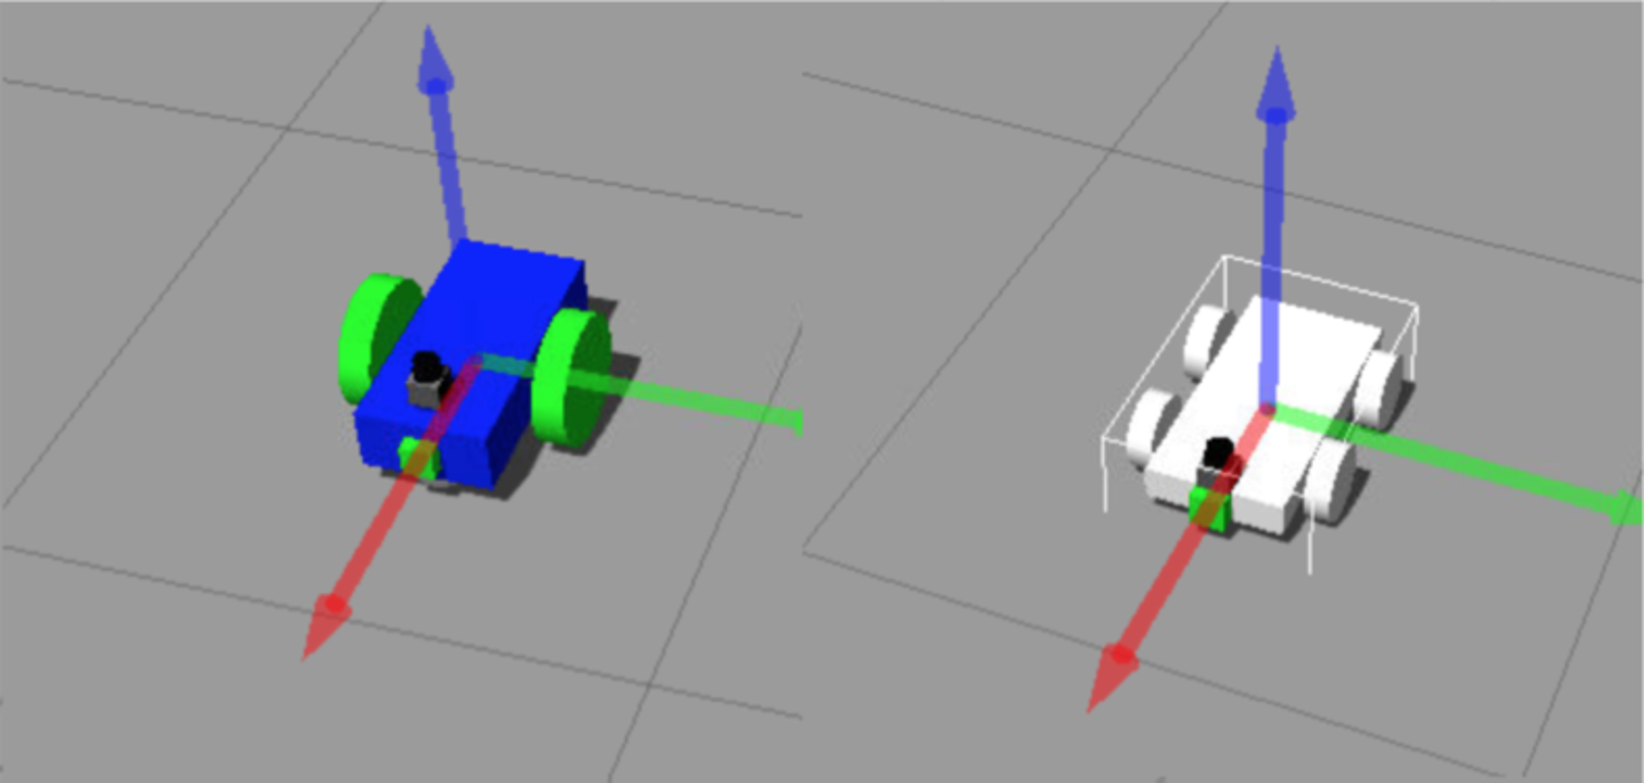
\includegraphics[width=\linewidth]{misc/intro.pdf}
      \caption{Mobile two- and four-wheeled robots.}
      \label{fig:intro}
\end{figure}

This project is focused on solving the global localization problem on a static environment, using a passive module, in a single-robot mobile platform. This has been implemented in simulation via ROS \cite{288} packages to illustrate navigation tasks (Fig. \ref{fig:intro}).  


%\IEEEPARstart{T}{he} introduction should provide some material regarding the history of the problem, why it is important and what is intended to be achieved. If there exists any previous attempts to solve this problem, this is a great place to note these while conveying the differences in your approach (if any). The intent is to provide enough information for the reader to understand why this problem is interesting and setting up the conversation for the solution you have provided
%Use this space to introduce your robotic inference idea and how you wish to apply it. 
%If you have any papers / sites you have referenced for your idea, please make sure to cite them.

%example for inserting image
%\begin{figure}[thpb]
%      \centering
%      \includegraphics[width=\linewidth]{RobotRevolution5}
%      \caption{Robot Revolution.}
%      \label{fig:robot1}
%\end{figure}

%\subsection{Subsection Heading Here}
%Subsection text here.
%
%\subsubsection{Subsubsection Heading Here}
%Subsubsection text here.
%
%
%\begin{table}[h]
%\caption{Table}
%\label{table_example}
%\begin{center}
%\begin{tabular}{|c||c|}
%\hline
%One & Two\\
%\hline
%Three & Four\\
%\hline
%\end{tabular}
%\end{center}
%\end{table}


\section{Background}

In global localization, the robot is placed within a known environment and localizes itself relative to an external reference frame. Due to the inherent uncertainty in sensor and motion measurements, the robot pose is represented by a \textit{belief}, a probability density function over the all possible locations and orientation.  Markov localization, an extension of the Bayes filter, provides a framework to obtain the robot pose as shown in the  Alg. \ref{alg:markov_localization}. 

\begin{algorithm}
\caption{Markov\_localization ($bel(x_{t-1}), u_t, z_t, m$)}\label{euclid}
\label{alg:markov_localization}
\begin{algorithmic}
\STATE  $\forall x_t$\textbf{:}
\STATE ~~~$\overline{bel}(x_t) = \int p(x_t | u_t, x_{t-1}, m)~bel(x_{t-1})~ dx_{t-1}$
\STATE ~~~$bel(x_t) = \eta~p(z_t | x_t, m)~\overline{bel}(x_t)$
\STATE \textbf{return} $bel(x_t)$
\end{algorithmic}
\end{algorithm}

The belief of the robot at time $t$ is represented by $bel(x_t)$. The measurement model and the motion model is given by $p(z_t | x_t, m)$, and $p(x_t | u_t, x_{t-1}, m)$ respectively. $u_t$ provides the control command to move the robot from time $t$-$1$ to t, while $z_t$ is the measurement, and $m$ is the static map of the environment. Kalman filter and Monte Carlo localization are two specific instances of the realization of the Alg. \ref{alg:markov_localization}, and further discussed herewith.   

\subsection{Kalman Filter Localization}
\label{sub:kfl}

The Kalman filter (KF) localization is a specific instance of Alg. \ref{alg:markov_localization}, the belief, measurement, and motion models are represented by the first (mean) and second (covariance) moments.  These assumptions limit the motion and measurement models to be linear, and the belief can only be represented by unimodal distribution such as a Gaussian. 

The practical systems are inherently non-linear, and the two common filters used in practice are the Extended Kalman filter (EKF), and the Unscented Kalman filter (UKF) localization. The EKF uses Taylor seriese expansion to linearize the non-linear model equations, while UKF uses sigma points for the transformation.  EKF and UKF localization represent with unimodal Gaussian and it is a good representation in uncertainty  for tracking problems, but generally not suitable for global localization. While  both algorithms addresses the limitation of the KF, the implementations use considerable computation resources (please refer to \cite{Thrun:2005:PR:1121596}, chapter 7, for comprehensive description of the filters).   

\subsection{Monte Carlo Location}
\label{sub:mcl}

Monte Carlo Localization (MCL) represents the belief $bel(x_t)$ of the robot pose by particles, which is a popular algorithm used in global and kidnapped robot localization.  MCL is computationally efficient than EKF and UKF, and it is not subjected to assumptions outlined in Sec. \ref{sub:kfl}. The basic steps of the MCL algorithm are:   \begin{enumerate*} \item the initial global uncertainty is achieved via a set of pose particles sampled uniform randomly over the entire pose space, \item the motion model moves the particles to the new locations, \item the measurement model assigns important factors to each particle based on the observations, \item the resampling setp samples particles relative to the importance weighs, and obtain the new belief, and set the new particles to uniform importance weights.  \end{enumerate*}

This project uses Adaptive Monte Carlo Localization  (AMCL) algorithm, which is a variant of MCL, that uses Kullback-Leibler divergence (KDL)-sampling to adapt the size of the particle set over time. 

\subsection{Practical Considerations}

Table \ref{tab:comp} summarizes and compares the localization algorithms discussed in Sec. \ref{sub:kfl} and \ref{sub:mcl}. While EKF and UKF are improvements over KF, they do come with limiting assumptions, and usage of considerable computational resources. On the other hand MCL and its variants can be used to represent multimodal distributions, and provide the ability to allocate proper computational resources.    

\begin{table}[h]
\caption{Comparison of EKF, UKF and MCL implementations}
\label{tab:comp}
\begin{center}
\begin{tabular}{|l||l|l|}
\hline
& EKF/UKF & MCL\\
\hline
Measurement & landmarks & row measurements\\
Measurement noise  & Gaussian & any\\
Posterior & Gaussian & particles\\
Efficiency (memory) & ++ &+\\
Efficiency (time) & ++ & +\\
Ease of implementation & + & ++\\
Resolution & ++ & +\\
Robustness & - & ++\\
Global localization & no & yes\\
\hline
\end{tabular}
\end{center}
\end{table}




%At this stage, you should begin diving into the technical details of your approach by explaining to the reader how parameters were defined, what type of network was chosen, and the reasons these items were performed. This should be factual and authoritative, meaning you should not use language such as “I think this will work” or “Maybe a network with this architecture is better..”. Instead, focus on items similar to, ”A 3-layer network architecture was chosen with X, Y, and Z parameters” 
%Explain why you chose the network you did for the supplied data set and then why you chose the network used for your robotic inference project. \cite{lamport1994latex}
%
%%example for Bullet point list
%
%\begin{itemize}
%\item example
%\end {itemize}



%example for numbered list
%\begin{enumerate}
%\item example
%
%\end{enumerate}

\section{Robot Simulation}

Robot Operating System (ROS) provides a set of tools and libraries to develop robot applications \cite{288}. Using ROS constructs, two mobile robots have been developed.  Rviz has been use for visualization, and Gazebo has been used as the simulator. 

\begin{figure}[thpb]
      \centering
      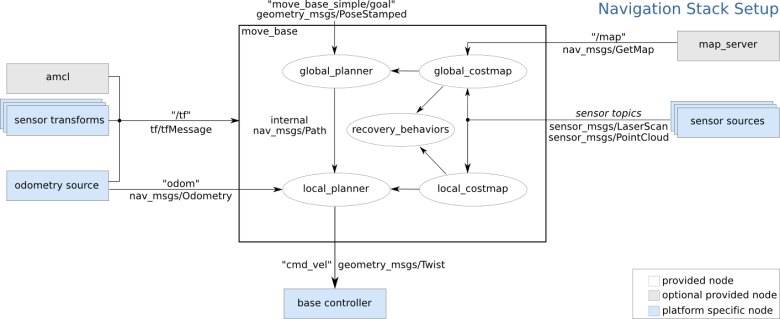
\includegraphics[width=\linewidth]{misc/overview_tf_small.png}
      \caption{amcl and navigation stack setup.}
      \label{fig:nav_stack}
\end{figure}

amcl\footnote{\url{http://wiki.ros.org/amcl}} package and navigation stack \footnote{\url{http://wiki.ros.org/navigation/Tutorials/RobotSetup}} have been installed in a catkin workspace and setup according to Fig. \ref{fig:nav_stack}. The simulation and parameter tuning were conducted on a Udacity virtual machine.

\subsection{Udacity Bot}

The baseline mobile robot, Udacity Bot, is developed using Xacro\footnote{\url{http://wiki.ros.org/xacro}} and Gazebo\footnote{\url{http://gazebosim.org/tutorials/?tut=ros_urdf}} definitions. The robot is two-wheeled robot equipped with a differential drive, Hokuyo laser scanner\footnote{\url{http://gazebosim.org/tutorials?tut=ros_gzplugins}}, and a camera. The structure of the robot is show in Fig. \ref{fig:udacity_bot}. The chassis is a 0.4, 0.2, 0.1 box, while the wheels are cylinder with radius 0.1 and length 0.05.  A differential drive has been attached to the left and right wheels, and configured via Gazebo file. 

\begin{figure}[thpb]
      \centering
      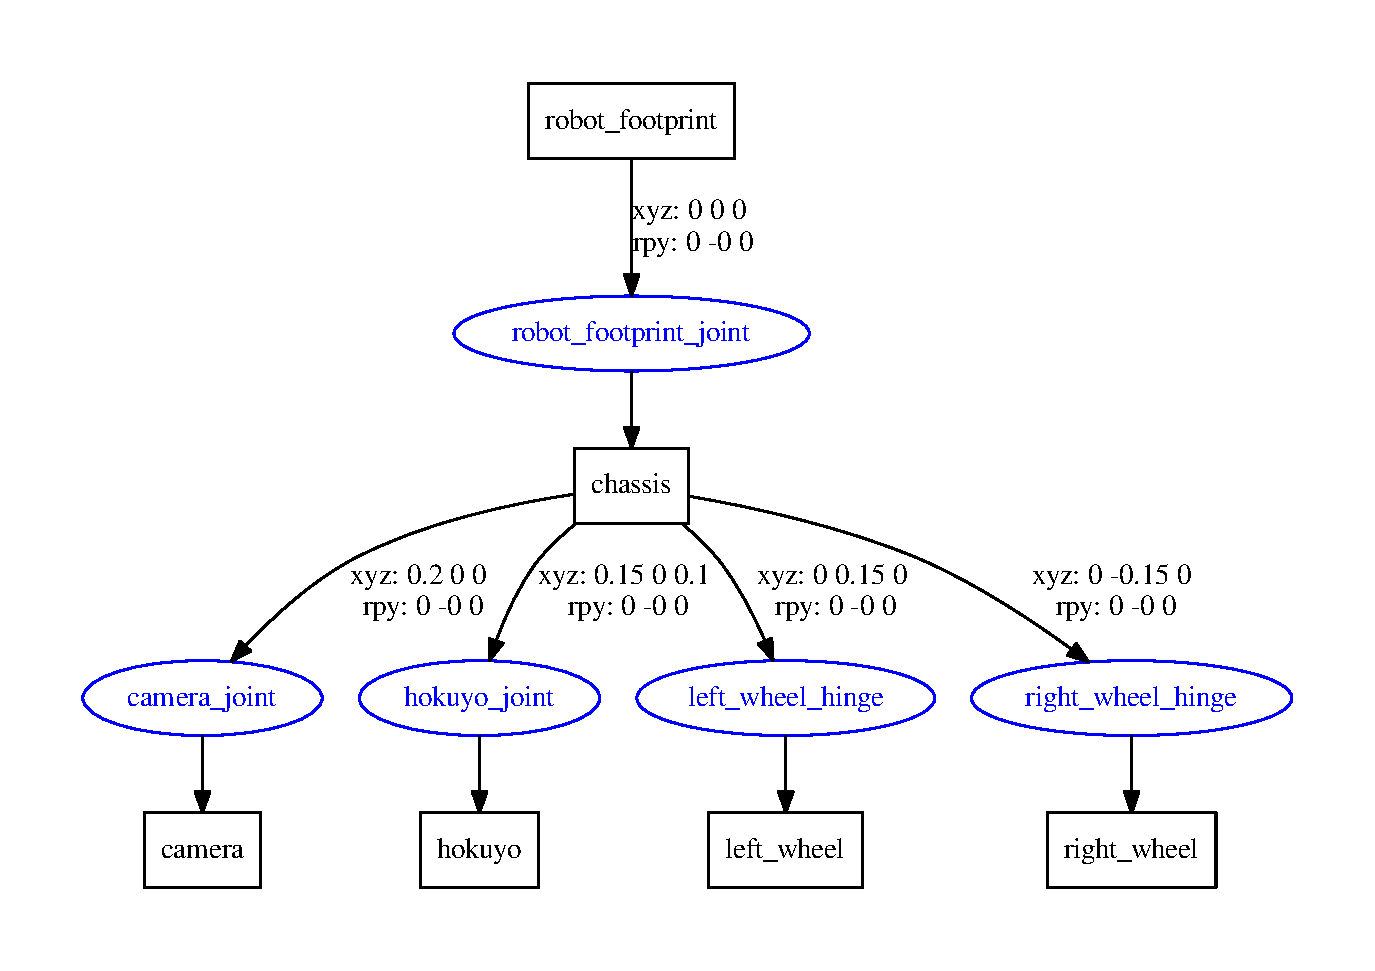
\includegraphics[width=\linewidth]{misc/udacity_bot.pdf}
      \caption{Structure of Udacity Bot.}
      \label{fig:udacity_bot}
\end{figure}




%\section{Data Acquisition}
%This section should discuss the data set. Items to include are the number of images, size of the images, the types of images (RGB, Grayscale, etc.), how these images were collected (including the method). Providing this information is critical if anyone would like to replicate your results. After all, the intent of reports such as these are to convey information and build upon ideas so you want to ensure others can validate your process.
%Justifying why you gathered data in this way is a helpful point, but sometimes this may be omitted here if the problem has been stated clearly in the introduction.
%It is a great idea here to have at least one or two images showing what your data looks like for the reader to visualize.

\section{Results}
This is typically the hardest part of the report for many. You want to convey your results in an unbiased fashion. If you results are good, you can objectively note this. Similarly, you may do this if they are bad as well. You do not want to justify your results here with discussion; this is a topic for the next session. 
Present the results of your robotics project model and the model you used for the supplied data with the appropriate accuracy and inference time
For demonstrating your results, it is incredibly useful to have some charts, tables, and/or graphs for the reader to review. This makes ingesting the information quicker and easier.

\section{Discussion}
This is the only section of the report where you may include your opinion. However, make sure your opinion is based on facts. If your results are poor, make mention of what may be the underlying issues. If the results are good, why do you think this is the case? Again, avoid writing in the first person (i.e. Do not use words like “I” or “me”). If you really find yourself struggling to avoid the word “I” or “me”; sometimes, this can be avoid with the use of the word “one”. As an example: instead of : “I think the accuracy on my dataset is low because the images are too small to show the necessary detail” try: “one may believe the accuracy on the dataset is low because the images are too small to show the necessary detail”. They say the same thing, but the second avoids the first person. 
Reflect on which is more important, inference time or accuracy, in regards to your robotic inference project.

\section{Conclusion / Future work}
This section is intended to summarize your report. Your summary should include a recap of the results, did this project achieve what you attempted, and is this a commercially viable product? 
For Future work,address areas of work that you may not have addressed in your report as possible next steps. For future work, this could be due to time constraints, lack of currently developed methods / technology, and areas of application outside of your current implementation. Again, avoid the use of the first-person.

\bibliography{bib}
\bibliographystyle{ieeetr}

\end{document}